\chapter{\Huge{LF8}}\label{ch:lf8}
\section{Datenbankentwicklung}\label{sec:lf8_first_Section}
\subsection{Einführende Bemerkungen zu Datenbanken}\label{subsec:einfuhrende-bemerkungen-zu-datenbanken}
\paragraph{Beantworten Sie die folgenden Fragen mit Hilfe des Textes "Einführende Bemerkungen zu Datenbanken" und der Recherche im Internet.}
\begin{enumerate}
    \item \color{brown}{Erläutern Sie den Unterschied zwischen Daten, Information und Wissen.}
    \begin{itemize}\color{black}
        \item \colorbox{yellow}{Daten:} In der Grundform sind Daten verschiedene Symbole und Zeichen, deren Bedeutung nur deutlich wird, wenn sie in einen Kontext gesetzt werden.
        Daten entstehen durch das Sammeln und Messen von Beobachtungen.
        \item \colorbox{yellow}{Information:} Die Daten gelangen auf eine komplexere Ebene und werden in Verknüpfung mit zusätzlichem Kontext zu einer Information.
        Informationen stellen Kenntnisse über Sachverhalte oder Personen dar.
        Es gibt verschiedene Ebenen, über die Informationsaustausch stattfinden kann.
        Je nach Sachlage und Kontext kann die Information relevant oder irrelevant sein.
        \item \colorbox{yellow}{Wissen:} Wissen beschreibt somit die gesammelten Informationen, die über einen bestimmten Sachverhalt oder eine Person zur Verfügung stehen.
        Um Wissen zu erlangen, müssen Informationen verarbeitet werden.
    \end{itemize}
    \item \color{brown}{Was versteht man unter einem Datenbankmanagementsystem DBMS?}
    \begin{itemize}\color{black}
        \item[] Ein \colorbox{yellow}{Datenbank-Managementsystem (DBMS)} ist eine Systemsoftware zum Erstellen und Verwalten von Datenbanken.
        Mit einem solchen Programm können Nutzer Daten in eine Datenbank einpflegen, um sie zu sammeln, lesen, aktualisieren und löschen.
    \end{itemize}
    \item \color{brown} {Welche Vorteile besitzt ein DBMS, welches das 3-Ebenen-Modell (ANSI-SPARC) als Grundlage hat.}
    \begin{itemize}\color{black}
        \item einfache Verwaltung großer Datensätze.
        \item einfacher, effektiver Zugriff auf gespeicherte Daten.
        \item hohe Flexibilität.
        \item Datenintegrität und -konsistenz.
        \item Zugriffskontrolle für Anwender (Datensicherheit und -schutz)
        \item hohe Verfügbarkeit\\
        \item[] Die Vorteile des \colorbox{yellow}{Drei-Ebenen-Modells sind:} Physische Datenunabhängigkeit: Die interne Ebene ist von der konzeptionellen und externen Ebene getrennt.
        Physische Änderungen, logische Datenunabhängigkeit: Die konzeptionelle und die externe Ebene ist getrennt.
    \end{itemize}
    \item \color{brown} {Fertigen Sie eine Skizze an, die das Zusammenspiel von Daten, Programmen und Benutzern in einem DBMS darstellt.}
    \begin{itemize}
        \begin{center}
            \begin{figure}[H]
                \centering
                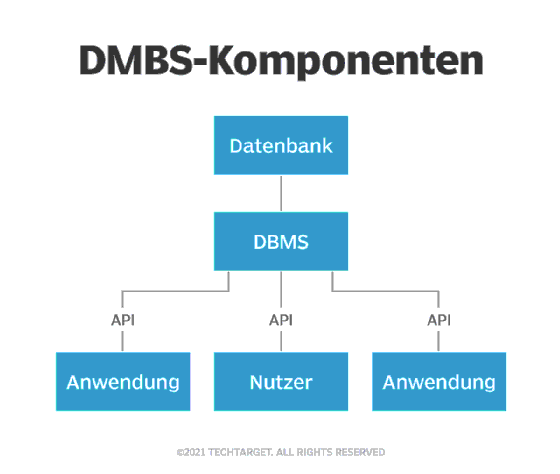
\includegraphics[height=5cm]{imgs/subjects_media/lf8/dmbs_compotents}
                \caption{\footnotesize Darstellung von Daten, Programmen und Benutzern in einem DBMS}\label{fig:DBMS}
            \end{figure}
        \end{center}
    \end{itemize}
    \item \color{brown}{Was versteht man unter Redundanz und Inkonsistenz?}
    \begin{itemize}\color{black}
        \item In der Informatik bedeutet \colorbox{yellow}{Inkonsistenz} von Daten Abweichung zwischen verschiedenen Daten.
        \item \colorbox{yellow}{Datenredundanz} bezeichnet die Praxis, Daten an zwei oder mehr Stellen in einer Datenbank oder einem Datenspeichersystem oder in mehreren geografisch entfernten Systemen zu speichern.
    \end{itemize}
    \item \color{brown}{Beschreiben Sie kurz die Entwicklungsgeschichte von Datenbanken.}
    \item \color{brown}{Welche DBMS sind zur Zeit auf dem Markt präsent und wie sind die Marktanteile verteilt (Internet nutzen)?}
    \begin{itemize}
        \begin{center}
            \begin{figure}[H]
                \centering
                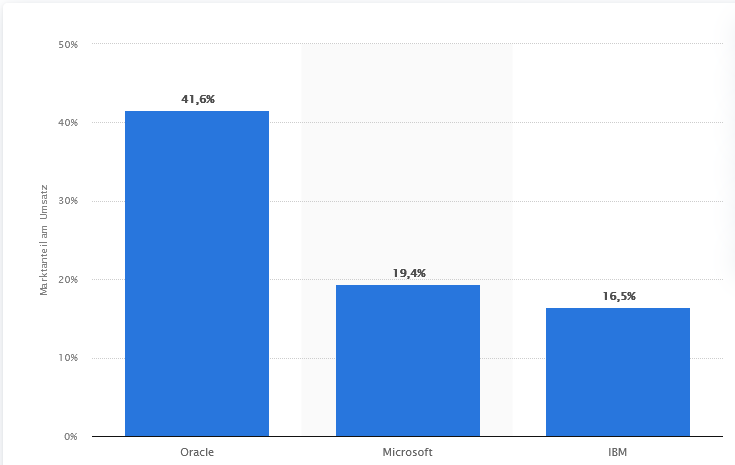
\includegraphics[height=5cm]{imgs/subjects_media/lf8/dmbs_marketanteil}
                \caption{\footnotesize Marktanteile der Anbieter am Umsatz mit Datenbankmanagementsystem-Software (DBMS) weltweit im Jahr 2015 }\label{fig:DBMS Marktanteile}
            \end{figure}
        \end{center}
    \end{itemize}
    \item \color{brown}{Was versteht man unter "Big Data", "Data Mining" und "Data Warehouse"?}
    \begin{itemize}\color{black}
        \item Der Begriff \colorbox{yellow}{„Big Data“} bezieht sich auf Datenbestände, die so groß, schnelllebig oder komplex sind, dass sie sich mit herkömmlichen Methoden nicht oder nur schwer verarbeiten lassen.
        Das Speichern großer Datenmengen oder der Zugriff darauf zu Analysezwecken ist nichts Neues.
        \item \colorbox{yellow}{Data Mining} ist die systematische Anwendung computergestützter Methoden, um in vorhandenen Datenbeständen Muster, Trends oder Zusammenhänge zu finden.
        Zur Wissensentdeckung eingesetzte Algorithmen basieren unter anderem auf statistischen Methoden.
        \item \colorbox{yellow} {Data Warehouse} - ein großes Lagersystem für Daten.
        Die Daten kommen aus unterschiedlichen Datenquellen des U. und werden in das Datawarehous übernommen.
        Diese Daten werden in den Datenbanken verwaltet.
        Die Daten werden hier langfristig gespeichert und stehen für diverse Analysen zur Verfügung.
        Die Daten können auch für die OLAP (Online Analytical Process) oder für die Data-Mining (gezieltes Suchen von Daten von Kunden mithilfe von Algorithmen) bereitgestellt werden.
    \end{itemize}
\end{enumerate}
\setcounter{section}{0}
\setcounter{figure}{0}